
\documentclass[12pt]{standalone}
\usepackage{amssymb,latexsym, amsmath,graphics}
\usepackage{amsthm}
\usepackage{setspace}

\doublespacing

\usepackage{pgf}
\usepackage{tikz}
\usetikzlibrary{arrows,automata}
\usetikzlibrary{positioning}



\begin{document}
\pagestyle{empty}
 \centering
 % Main layout borrowed from 
 % Gray Code in 4-cube
% Author: Yury Chebiryak <http://yury.chebiryak.name/index.html>
%\documentclass{article}
%\usepackage{tikz}

 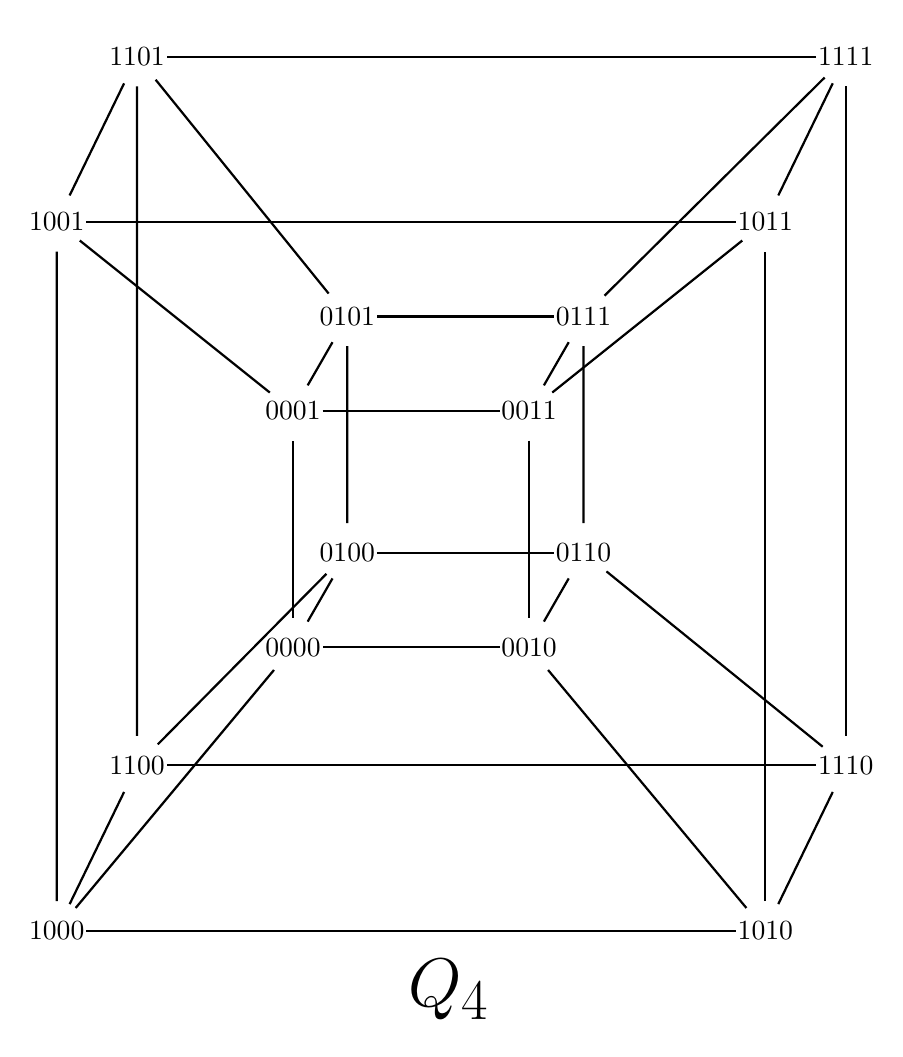
\begin{tikzpicture} [scale=3]
	 \tikzstyle{vertex}=[circle,minimum size=20pt,inner sep=0pt]
	 \tikzstyle{edge} = [draw,thick,-,black]
%	 \node[vertex] (v0) at (0,0) {$0000$};
%	 \node[vertex] (v1) at (0,1) {$0001$};
%	 \node[vertex] (v2) at (1,0) {$0010$};
%	 \node[vertex] (v3) at (1,1) {$0011$};
%	 \node[vertex] (v4) at (0.23, 0.4) {$0100$};
%	 \node[vertex] (v5) at (0.23,1.4) {$0101$};
%	 \node[vertex] (v6) at (1.23,0.4) {$0110$};
%	 \node[vertex] (v7) at (1.23,1.4) {$0111$};
	 \node[vertex] (v0) at (0,.2) {$0000$};
	 \node[vertex] (v1) at (0,1.2) {$0001$};
	 \node[vertex] (v2) at (1,0.2) {$0010$};
	 \node[vertex] (v3) at (1,1.2) {$0011$};
	 \node[vertex] (v4) at (0.23, 0.6) {$0100$};
	 \node[vertex] (v5) at (0.23,1.6) {$0101$};
	 \node[vertex] (v6) at (1.23,0.6) {$0110$};
	 \node[vertex] (v7) at (1.23,1.6) {$0111$};
	 
	 \node[vertex] (v8) at (-1,-1) {$1000$};
	 \node[vertex] (v9) at (-1,2) {$1001$};
	 \node[vertex] (v13) at (-0.66,2.7) {$1101$};
	 \node[vertex] (v12) at (-0.66,-0.3) {$1100$};
	 \node[vertex] (v10) at (2,-1) {$1010$};
	 \node[vertex] (v14) at (2.34,-0.3) {$1110$};
	 \node[vertex] (v11) at (2,2) {$1011$};
	 \node[vertex] (v15) at (2.34,2.7) {$1111$};
	 
	 \draw[edge] (v0) -- (v1) -- (v3) -- (v2) -- (v0);
	 \draw[edge] (v0) -- (v4) -- (v5) -- (v1);
	 \draw[edge] (v2) -- (v6) -- (v7) -- (v3);
	 \draw[edge] (v4) -- (v6);
	 \draw[edge] (v7) -- (v5);
	 
	 \draw[edge] (v8) -- (v9) -- (v13) -- (v12);
	 \draw[edge] (v4) -- (v12) -- (v8) -- (v0);
	 \draw[edge] (v1) -- (v9);
	 \draw[edge] (v13) -- (v5);
	 \draw[edge] (v2) -- (v10) -- (v14) -- (v6);
	 \draw[edge] (v8) -- (v10);
	 \draw[edge] (v14) -- (v12);
	 \draw[edge] (v3) -- (v11) -- (v15) -- (v7);
	 \draw[edge] (v10) -- (v11);
	 \draw[edge] (v15) -- (v14);
	 \draw[edge] (v9) -- (v11) ;
	 \draw[edge] (v15) -- (v13);
	 
	 
	 
	 \node[] at (.66,-1.25) {\Huge $Q_4$};
 \end{tikzpicture}
\end{document}